\documentclass[12pt]{article}

\usepackage[toc,page]{appendix}
\usepackage{graphicx}
\usepackage{float}
\usepackage[T1]{fontenc}
\usepackage{ulem}
\usepackage{amsmath}
\usepackage{amssymb}
\usepackage{caption}
\usepackage{enumitem}
\usepackage[left=2.90cm, right=2.90cm, top=3.30cm, bottom=4.20cm]{geometry}
\usepackage{parskip}

\setlength{\parskip}{11pt plus4mm minus3mm}



\DeclareCaptionFont{smaller}{\fontsize{9pt}{9pt}}
\captionsetup{singlelinecheck=off, font=footnotesize}
\setlength{\footskip}{43pt}


\title{Group Report for Computing Assignment: The Cell Behaviour Modelling Platform}
\author{Ryan Carey, Lewis Kindeleit, Antoine Messager}

\begin{document}

\maketitle
{\centering
\subsubsection*{M Sc Bioinformatics and Theoretical Systems Biology 2014-15}
\subsubsection*{Supervisor: MPH Stumpf} 
\subsubsection*{Word Count: 6923}
}

\newpage
\tableofcontents
\newpage
\section{Introduction --- written by LK and RC} 
Agent-based models (ABMs) are suited to simulating cellular dynamics because the behaviour of cells can 
depend on their complex interactions.\cite{kaul15} By implementing the rules 
that dictate the behaviour of the smallest components of biological systems it is possible to analyse the emergent 
behaviour to see if the researcher’s understanding is correct. This agent-based approach has gained popularity in recent 
years as increases in computing power have allowed for more sophisticated behaviour to be simulated. 
This in turn has increased the relevance of output data, improving the scope for using them to inform 
future experimental direction. \cite{grimm06} \cite{drasdo07}

To this end, ABMs have been created to analyse a myriad of biological problems such as cell migration 
and tumour formation with varying degrees of success. However, the technical expertise required to 
create such a model limits the amount of biologists who utilise these useful tools. An adaptable and 
easy-to-use platform could potentially assist many experimental biologists to test formal models for 
how observed cells behave. The long-range goal to decrease the barriers to  ABM creation for researchers 
was the basis for our platform, the Cell Behaviour Modelling Platform (CBMP).

The CBMP is a research tool that can simulate a variety of systems in which cells move through continuous 
space in response to diffusing environmental stimuli and each other. It can be used to create kinds of 
cells and environmental stimuli, where the cells behave according to user specified parameters. In the absence 
of environmental stimuli, the cells walk according to a combination of persistence and 
randomness, according to walk models that have a long history of use in biology.\cite{codling08} 
When environmental stimuli are present, cells decide where to move based on several factors: 
the evaluation of chemical stimuli, the cells current direction of motion and a random component. The 
growth of cells depends on whether they have sufficient space around them. The model implements simple 
rules describing how cells interact with each other and their environment, which gives the opportunity 
to observe emergent behaviour and to compare this to real world experimental data. This comparison can 
be used to check whether the mechanics underlying the simulation are approximately correct or to discover 
previously unknown characteristics about the system undergoing investigation.

The platform has been developed in Julia, a relatively new language that is highly optimized for performance 
but nonetheless offers readable syntax and short development time. This has resulted in a platform that 
can simulate many individual cells within a continuous space environment at good speed, whilst still 
being very accessible and easily modified to suit new users’ needs. This means the platform is an easily 
accessible tool that has a large amount of room to be tailored to an individual's preferences. The platform 
is intended to gain functionality via new users implementing code that suits their specific needs. Extending 
the platform in this manner is substantially less difficult and time-consuming than designing an ABM 
from scratch. The CBMP allows substantially varied models. Moreover the codebase is designed to tolerate 
significant customisation and is made publicly available online. The intent is for the CBMP to facilitate 
inferences about many of the diverse cellular systems being investigated today.

In the absence of an environmental stimulus, the cells carry out a walk 
that includes elements of persistence and randomness. When environmental 
stimuli are present, cells decide where to move based on several 
factors: the evaluation of chemical stimuli, the cell's current 
direction of motion and a random component. The growth of cells depends 
on whether they have sufficient space around them. The model implements 
simple rules describing how cells interact with each other and their 
environment, which gives the opportunity to observe emergent behaviour 
on the simulation and to compare this to real world experimental data. 
This comparison can be used to check whether the mechanics underlying 
the simulation are approximately correct or to discover previously 
unknown characteristics about the system undergoing investigation.

\section{Installation --- written by RC and LK}
The CBMP has been developed in Julia 0.4. in RedHat Enterprise Linux 
Workstation release 6.2, and has also been tested on Ubuntu 14.04 in 
Julia 0.3. The platform should run on any operating system 
that has Julia installed, however there may be slight differences 
between them.

To run the CBMP, first Julia must be installed. If this has already been 
done, please skip to the Dependencies section.

\subsection{Detailed Instructions}
To install Julia, follow the instructions on the website, 
http://julialang.org/downloads/. Similarly,
install Python at www.python.org/downloads if you do not have it already. 
The Julia packages Winston, Tk and PyCall are most easily installed 
using the interactive Julia prompt. The Julia prompt is opened by entering
into the command line: \\

{\fontsize{11pt}{11pt} \ttfamily 
> julia} \\

To install the required packages, enter the following into Julia's interactive prompt: \\

{\fontsize{11pt}{11pt} \ttfamily 
> Pkg.add("\,Winston") \\

> Pkg.add("\,Tk") \\

> Pkg.add("\,PyCall")} \\ 

To return to the command line, enter: \\

{\fontsize{11pt}{11pt} \ttfamily 
> exit()} \\

You can install the python package {\itshape Pickle} by typing into the command line: \\

{\fontsize{11pt}{11pt} \ttfamily 
> pip install pickle} \\

If all of the dependencies are already installed, then all you need to 
do is download the repository and run CBMP.jl.

\subsection{Dependencies}

The installation depends on:

\begin{itemize}
  \setlength\itemsep{1em}
\item Julia 0.3 -- 0.4 with:
\begin{itemize}
  \setlength\itemsep{1em}
\item Winston
\item Tk
\item PyCall
\end{itemize}
\item Python (tested on 2.8 and 3.4 but it should work for other 
versions) with:
\begin{itemize}
  \setlength\itemsep{1em}
\item Pickle
\end{itemize}
\end{itemize}

Once you have installed the dependencies, all you need to do is download 
the repository and run CBMP.jl. If you have git installed, you do this 
by entering into your command line: \\

{\fontsize{11pt}{11pt} \ttfamily 

> git clone https://github.com/RyanCarey/abm-platform.git \\

> julia CBMP.jl} \\

The software comes with 2 different methods of inputting parameters and 
starting simulations: an easy to use GUI and a command line version. The 
GUI has been created with experiment design in mind; it gives the user 
fine-grained control of all parameters that describe the behaviour of 
cells and the way in which environmental stimuli diffuse through the 
environment, whilst providing immediate feedback.

The command line version, whilst being more complicated to operate, is 
much faster at performing simulations due to the lack of simulation 
display and increased parameter input speed. Parameters are input 
directly into the code and as such requires slightly more expertise to 
use. This option is intended to be used when experimental setup is 
already decided and multiple simulations are required to be run to 
collect data.

\subsection{The Graphical User Interface}
The overall structure of the graphical user interface is that of a main 
menu that controls the most important parameters, and three submenus 
that are used to control the details pertaining to diffusion, cell types 
and borders. Help buttons are available in all menus to provide 
detailed instruction on the function of each parameter.

\subsubsection{Main Menu}
The main menu allows the user to alter environment-wide parameters such 
as starting number of cells and the size of the environment (Figure 1). 

\begin{figure}[H]
\centering
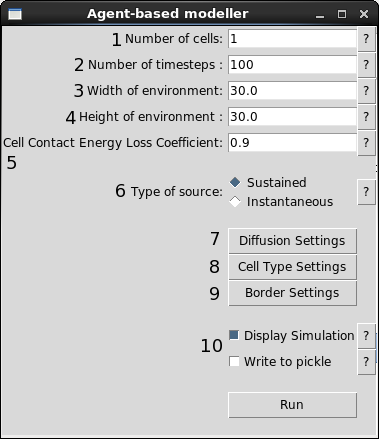
\includegraphics[width=7.99cm]{media/main_screen_annotated.png}
\caption[]{The program's main screen, which contains settings 
for some of the major features of the model, and has buttons which open 
detailed settings. The settings are:

\begin{enumerate}[topsep=2pt,itemsep=-1ex,partopsep=1ex,parsep=1ex]
\item {\itshape Number of cells:} The total number of cells at the start 
of the simulation.
\item {\itshape Number of timesteps:} The number of iterations made by 
the simulation before the simulation is terminated. At each iteration, 
one randomly chosen cell is updated.
\item {\itshape Width of Environment:} This denotes the width of the 
simulation environment in some arbitrary units.
\item {\itshape Height of Environment:} This denotes the height of the 
simulation environment in some arbitrary units.
\item {\itshape Energy Loss Coefficient:} This specifies the factor by 
which cellular momentum is multiplied upon each contact event.
\item {\itshape Type of Source:} Allows the user to choose between 
a sustained and instantaneous source.
\item {\itshape Diffusion Settings:} Opens the diffusion settings menu. See Diffusion Menu below.
\item {\itshape Cell Type Settings:} Opens the menu for altering cell 
type settings. See Cell Types below.
\item {\itshape Border Settings:} Opens the border menu. See Border Menu below.
\item {\itshape Display / Write:} Selecting these options will display 
the simulation if desired and allow an output of the results of the 
simulation to be saved to file as a binary 'pickle' file. Note that 
displaying the simulation slows the process considerably, and should be 
turned off for long simulations.
\end{enumerate}
}
\end{figure}

\newpage
\subsubsection{Diffusion Menu}
The diffusion menu (shown in Figure 2) contains the settings that control how 
ligand will spread through the environment. The results of 
tuning the diffusion parameters can be visualised and controlled 
interactively using a slider.

\begin{figure}[H]
\centering
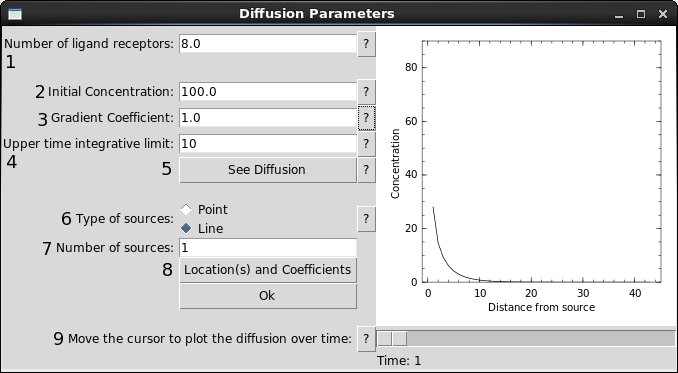
\includegraphics[width=13.51cm]{media/diffusion_screen_annotated.png}
\caption[]{The diffusion menu, which contains 
settings for controlling the how ligand diffuses through the cells'
environment. On the right is a graph that shows how the 
concentration gradient will change over time, where time is 
interactively changed using the slider in the lower right. The diffusion 
menu settings are as follows:
\begin{enumerate}[topsep=2pt,itemsep=-1ex,partopsep=1ex,parsep=1ex]
  \item {\itshape Ligand Receptors:} 
      The number of points on the cell 
  surface where ligand concentration is sampled. These are evenly spaced 
  out along the cell surface.
  \item {\itshape Initial Concentration:} This is the A coefficient in the 
  diffusion equation. Increasing this number proportionally increases the 
  ligand concentration. Note that this coefficient 
  does not affect the simulation and is only used for the graphical display.
  \item {\itshape Gradient Coefficient: }This is the D coefficient in the 
  diffusion equation. It is usually called the diffusion coefficient. 
  Decreasing this number will increase the slope of the diffusion. It is 
  equivalent to reducing the time of diffusion. Note that this coefficient 
  does not affect the simulation and is only used for the graphical display.
\item {\itshape Time Limit:} This is \(\tau\) in the diffusion equation. 
  It defines when the source will cease to emit ligand. This parameter 
  is only available if sustained diffusion is selected. Note that this 
  entry is only used for visualisation. To create a source for the model,
  click Locations and Coefficients.
  \item {\itshape See Diffusion:} Updates the graph to the right with the 
  parameters specified in 2-4. 
  \item {\itshape Type of source:} Select the type of source.
  \item {\itshape Number of sources: }The total number of sources present 
  in the simulation from the start.
  \item {\itshape Locations and Coefficients: }Allows the user to select 
  the locations of each possible source, and change its characteristics. 
  For more information see below.
  \item {\itshape Diffusion Over Time:} Displays the 
  diffusion over space and time as per the coefficients given in 2-4.
\end{enumerate}
}
\end{figure}

\subsubsection{Source Location Menu}
The source menu (in Figure 3) controls where the ligand is emitted 
from, for how long, and with what gradient.

\begin{figure}[H]
\centering
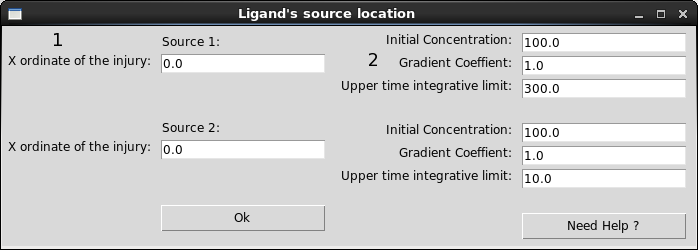
\includegraphics[width=13.51cm]{media/source_loc_screen_annotated.png}
\caption[]{The source menu, which allows the user to specify 
where ligand comes from, and how it is produced.
\begin{enumerate}[topsep=2pt,itemsep=-1ex,partopsep=1ex,parsep=1ex]
\item {\itshape Location:} the source location is specified here. In the 
case of a line source, this is a single x-ordinate. In the case of a 
point source, x- and y-ordinates would be shown..
\item {\itshape Parameters:} Allows each individual ligand source to be 
customised, following the rules described under Diffusion Menu.
\end{enumerate}
}
\end{figure}

\subsubsection{Cell Type Menu}
The cell type menu controls most of the complexity of the CBMP's models 
by allowing a wide range of parameters for up to four cell types (Figure 
4). 

\begin{figure}[H]
\centering
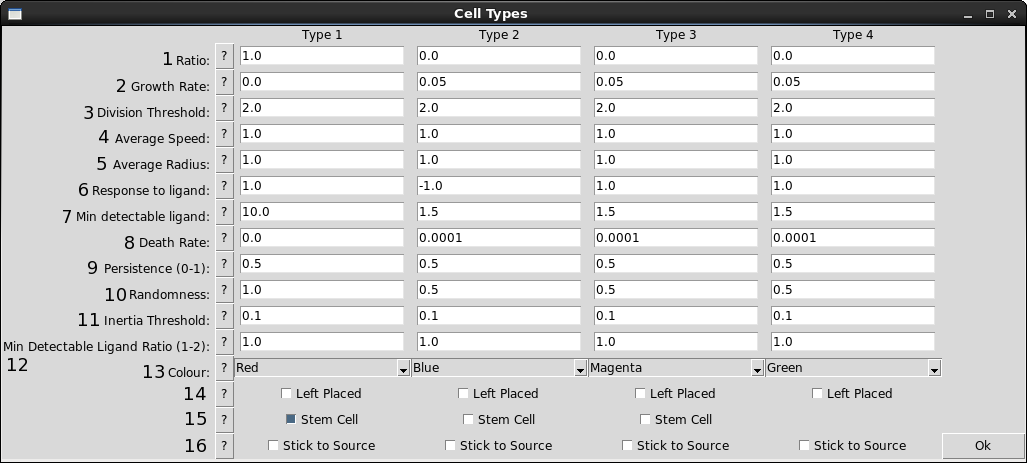
\includegraphics[width=\textwidth]{media/cell_type_screen_annotated.png}
\caption[]{The cell type window, which allows the user to 
specify parameters for each of the four cell types. The parameters are:
\begin{enumerate}[topsep=2pt,itemsep=-1ex,partopsep=1ex,parsep=1ex]
\item {\itshape Ratio:} The relative amount of this type of cell.
Ratios are normalised and as such do not have to sum to one.
\item {\itshape Growth Rate:} The rate at which a cells area will 
increase per timestep.
\item {\itshape Division Threshold:} The ratio of initial area to 
initial area at which a cell division event will occur.
\item {\itshape Average Speed:} The average distance a cell travel
in one step.
\item {\itshape Average Radius:} The average radius of cells at the 
start of a simulation.
\item {\itshape Ligand Response:} The sign of the ligand response 
  determines whether cells are attracted (positive) or repelled (negative)
  from the source.
\item {\itshape Min Detectable Ligand:} This defines whether a cell
  can detect the ligand, and equivalently whether it believes it is in 
  a stem cell niche.
\item {\itshape Death Rate:} The chance that at any time step, the cell will die.
\item {\itshape Persistence:} The fraction of a cell's move that is 
derived from its last move.
\item {\itshape Randomness:} The fraction of a cells move that is random.
\item {\itshape Inertia Threshold:} The minimum speed at which colliding cells continue to move.
\item {\itshape Min Detectible Ligand Ratio:} The ratio of maximum ligand 
concentration to mean ligand concentration detected by individual cells 
receptors. If the ratio is below this value, the signal is 
deemed to be lost to noise, and the cell will not respond to it.
\item {\itshape Colour:} Possible cell type colours are: Red, Blue, Magenta, Green and 
Yellow.
\item {\itshape Special Options:} These represent specific special 
functions cell types can have.
\item {\itshape Left Placed:} If checked, these cells are initialised at the left wall of the environment.
\item {\itshape Stem Cell:} If checked, these cells change the type of their progeny depending upon local ligand 
concentration. Progeny are either of the same type (stem cell replication), or the subsequent type  
(\(1 \rightarrow 2 \rightarrow 3 \rightarrow 4\)). Note that type 4 cells cannot be stem cells. If not checked,
cells divide to produce only cells of their own type.
\item {\itshape Stick to Source:} Causes cells of this type to slow down by 90\% when they can detect
  a large amount of ligand in their environment, effectively sticking them in place.
\end{enumerate}
}
\end{figure}

\subsubsection{Border Menu}
The last menu is the borders menu, which allows the user to decide which 
individual borders will respond to cells by reflecting, absorbing or 
removing them. Its controls are detailed in Figure 5.

\begin{figure}[H]
\centering
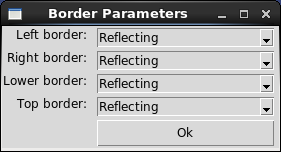
\includegraphics[width=6.13cm]{media/border_screen.png}
\caption[]{The border menu Each of the four 
borders can independently be set to perform reflecting or absorbing 
collisions, or to remove cells.}
\end{figure}

\subsection{The Interactive Prompt Interface}
Alternatively, the CBMP can be accessed from Julia's interactive prompt. 
The command line option is intended to be used as a way of performing 
multiple identical simulations in order to collect data. As such the 
option to visualise simulations is disabled, and the option to save data 
to file is enabled by default. In order to run the CBMP in the command 
line, the user should simply type in the terminal: \\

{\fontsize{11pt}{11pt} \ttfamily 

> julia (to enter the REPL) \\

> include("\,run\_sim.jl") \\

> run(Number of Simulations; {\itshape[type="Optional\_Preset\_Parameter"]})}\\

The command-line argument specifies the number of simulations. Any 
simulation specific parameter changes can be made in the file 
``run\_sim.jl''. This approach to parameter customisation was made in 
light of the amount of parameters that can be altered, as it would be 
unfeasible to include all parameters as function arguments. Any 
parameter that can be changed within the GUI is available for alteration 
within the command line version. If the user desires to replicate the 
simulations we discuss later, the command line version can be run with 
an additional function argument. These are ``niche\_sim'', ``migrate\_random'' 
and ``migrate\_non\_random''. These presets already have the parameters 
that our simulations ran saved within them. The user can copy this code 
and substitute parameters to store their own simulations.

Comments are provided in {\itshape run\_sum.jl} so that users can see 
what different parameters do. These parameters are laid out similarly to 
the graphical menus (For instance, the cell type characteristics are 
shown in run\_sim.jl), and are written as Julia variables (Figure 6).

\begin{figure}[H]
\centering
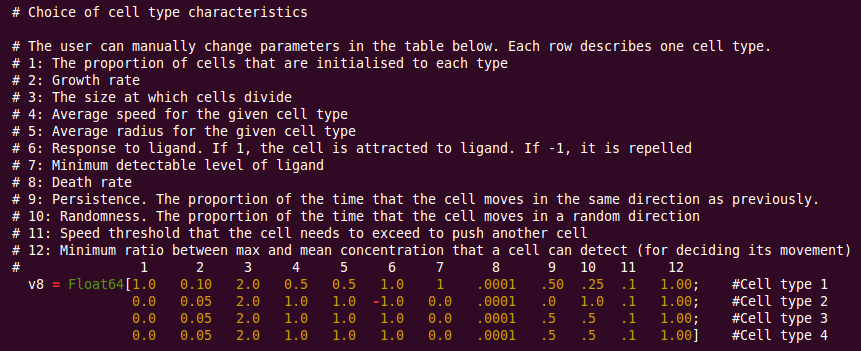
\includegraphics[width=\textwidth]{media/runsim.png}
\caption[]{Source code for run.jl: choosing cell type parameters}
\end{figure}

\subsection{Accessing Binary Outputs}
Instead of viewing simulations on the graphical display, they can be 
stored to be used later. To reduce storage space, these are stored as 
binary files using Python's ``Pickle'' module (Pickle is in turn called 
using Julia's PyCall). Since it would be highly redundant to store the 
locations of all cells at every timestep, the locations of every cell 
are by default stored every 250 timesteps. Each pickle file documents 
the time that the simulation took place and the all parameters used.

This pickle file can easily be unpacked into an array in Julia or 
Python. In each language, this is done using an ``unpickle'' function 
that is provided in the repository in the ``unpickle.jl'' and 
``unpickle.py'' files respectively. In Python, further utilities are 
provided in ``unpickle.py'' for conveniently processing a series of 
simulations. ``get all'' can take the list of filenames printed out by 
the command line utility and store the cell positions in each simulation 
in an array. ``stack'' can be further used to combine the simulations 
together into one time series. All of these are provided for 
conveniently analysing the output from the CBMP.

\section{The Model}
The framework of the model can be seen briefly outlined in Figure 7. To 
begin with, cells are allocated to non-overlapping locations using 
sequential random placement. If not all cells can be placed in the size 
of environment specified, the model will stop trying to place cells and 
report this. However, the simulation will then begin with the amount of 
cells that had already been placed. Once completed, the simulation will 
then iterate over five steps for the amount of user-specified time. 
These events take place in two-dimensional continuous space. 

\begin{figure}[H]
\centering
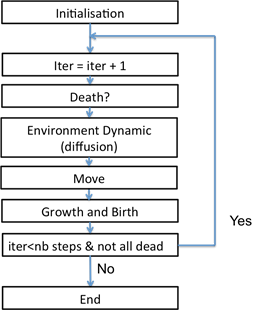
\includegraphics[width=5.81cm]{media/algorithmoverview.png}
\caption[]{Global overview of the model. The three stages of the program
  are initialisation (green), iteration (blue) and termination (red). 
  Interation has five parts: cell death, environment dynamic, movement, cell 
growth and mitosis.}
\end{figure}

\subsection{Initialisation --- written by RC, software developed by AM and RC}
The agents are placed in a rectangular environment, in which space is 
continuous and time advances in discrete timesteps. The cells are 
positioned randomly, either on one edge of the environment (as with 
haematopoietic stem cells in a niche model), or across the whole field, 
depending upon their specified type location. If a proposed location 
overlaps with another cell, then a new location is randomly generated 
and proposed (random sequential placement). If many attempts are made to 
fit a cell in the given field but the cells are simply too numerous or
too large, then the simulation stops placing new cells and carries out 
the simulation with the amount of cells it had so far placed correctly.

The cells are modelled as agents with rigid, circular edges of varying 
radius. Each cell has a type, which determines its behaviours. Cells of 
the same type grow, move and divide at similar rates with a slight 
individual randomness. However, they differ in their physical 
characteristics --- their radius, location and direction of travel.

\subsection{Iteration}
Once the cells are placed, one cell is selected for action each turn. 
This cell proceeds through the four major cellular functions: death, 
movement, growth and division. The cellular functions performed by the 
platform try to encapsulate most of the basic behaviours of cells. There 
is scope within the platform for the way these behaviours are 
implemented to be changed or removed, or new behaviours added.

\subsubsection{Cell Death --- written and developed by LK}
Cell death is modelled as random, and uniform for a given type of cell. 
This assumes that cell death is independent of the cells' environment, 
and in particular, independent of prior deaths that have occurred in 
that cell's vicinity. In reality, apoptosis is mediated by environmental 
factors, and this could be included with the development of a more 
sophisticated environmental model.

\subsubsection{Movement --- written by AM and RC and developed by AM}
When a cell moves, it is stochastically assigned a vector that 
determines its change in position from timestep n to timestep n+1. If 
the cell's proposed position at time n+1 overlaps with another cell, or 
with the wall, then the overlap-resolving function is called and it 
tentatively suggests a new movement vector for that cell and any other 
cells that it collides with. The alternative movement vectors are then 
checked recursively for collisions.

The magnitude of the initial movement vector is drawn from a Chi-squared 
distribution with two degrees of freedom. 

A cell's movement is determined by three aspects: the ligand, the 
randomness and the persistence. These are each explained in turn.

In order to decide where to move, cells detect the amount of ligand at 
receptor locations on their cell membrane. In the model, the number of 
receptors is parameterised by the user, and these receptors are spaced 
equally around the circumference of the cell. 

The cell is then most likely to go in the direction that - according to 
its receptors - has maximal concentration. Since it would not be 
biologically realistic for a cell to reliably filter infinitesimal 
differences in concentration from noise, the user is allowed to 
decide the minimum ratio (and also a minimum absolute amount) of ligand 
that cells are able to detect. In the case of a stem cell, this 
threshold is also used to indicate whether the stem cell is in the 
niche, and this determines its mitotic behaviour.

If the cell cannot detect the surrounding ligand, its motion is 
determined by a combination of its last movement vector and random 
chance. This combination is weighted by user-specified persistence and 
randomness parameters.

When a movement is proposed for a cell, there are two ways that its 
movement can be interrupted: by collision with the wall, or by collision 
with another cell. If a cell is reflected off the wall, then it bounces 
of the wall as per the border parameterization, and this new movement 
vector is assessed for any overlaps. If there is overlap with another 
cell, then both cells bounce off each other, and their new movement 
vectors are assessed for overlap. These new movements are checked 
recursively until all cells are placed in non-overlapping locations and 
the movement phase concludes.

\subsubsection{Growth and Division --- written and developed by LK}
Cells grow according to a user specified growth rate that depends on the 
cell's area. Because only one cell grows per timestep, the growth rate 
is adjusted to account for the number of cells in the simulation. 
Whether a cell divides depends on two factors: i) the ratio of its size 
to the size at which that type of cell is initialised (if this ratio 
exceeds the specified threshold then the cell will divide) and ii) the 
adjacent space available. If there is insufficient space to place two 
daughter cells, then the cell will refrain from dividing. When cells 
divide, each of the daughter cells have half of the area of the parent 
cell. 

To model stem cells, rules have been specified to determine which 
daughter cells they will give rise to. For stem cells, if the local 
ligand concentration is above the user-specified threshold, then 
division is likely to produce two stem cells. If the concentration is 
below the threshold, the division will result in one or both of the 
daughter cells becoming progenitor cells instead.

The CBMP allows generation of ligand as an instantaneous pulse, or 
continuously over finite time. There can be multiple sources, so long as 
they are all of the same variety. Modelling how cells are affected by 
ligand depends on modelling its diffusion. These environmental 
models are best understood by beginning with the instantaneous case.

\subsubsection{Diffusion --- written by AM and RC, developed by AM and RC}
{\bfseries Instantaneous Pulse of Ligand} \\
The equations governing the diffusion of ligand from an instantaneous 
source can be derived from the example of a single particle \(P\) that can 
move along an axis, as in Figure 8.

\begin{figure}[H]
\centering
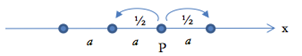
\includegraphics[width=9.28cm]{media/particlep.png}
\caption[]{A particle moving stochastically through 
one-dimensional space}
\end{figure}

The particle \(P\) is taken to have an equal probability of 
moving left or right. Let the length of each jump be \(a\), and 
the time elapsed during each jump be \(\tau\), and assume that 
the particle takes another step immediately as soon as each previous 
step has concluded. Assume that at time 
\(t=0\), the particle is located at \(x=0\). After \(N\) jumps of which \(n\) are in a 
leftwards direction, the particle will be located at \(x_n = N-2n\). 
After \(N\) jumps, there are \(\binom{N}{n}\) ways 
for the cell to end up at \(x_n\) of \(2^N\) possible moves in 
total, therefore the probability of being located at \(x_n\) is:
\begin{equation} 
  p(x_n,t_N) = \frac{\binom{N}{n}}{2^N} = \frac{N!}{2^N(\frac{N-n}{2})!(\frac{N+n}{2})!}
\end{equation}

If the timestep size is small, (\(\tau \ll 1\)) and the number of timesteps is large, 
(\(N \ll 1\)), then our model increasingly resembles continuous time. 
In the limit, using Sterling's approximation 
and some algebra, this gives a continuous model that is continuous in 
time, as per Fick's Law.\cite{fick55}

\begin{equation}
  p(x_n,t_N) = \sqrt{\frac{1}{2\pi N}}\exp(-\frac{n^2}{2N}) = \sqrt{\frac{\tau}{2\pi t}}\exp(-\frac{\tau x^2_n}{2a^2t})
\end{equation}

The last expression still includes a spatial parameter, which was 
previously taken to be discrete: 

\begin{equation}
  \delta = \sqrt{\frac{a^2t}{\tau}}
\end{equation}

However, we can assume that \(\delta \gg a\), and therefore the 
model will be correct in continuous space. The probability of being at 
time \(t\) between \(x\) and \(x+dx\) with \(\delta \gg dx \gg a\) is:

\begin{equation}
  dp = \frac{dx}{a}p(x,t)
\end{equation}

If we let \(D = \frac{a^2}{2\tau}\), then \(dp\) can be expressed as a 
function of \(x\), \(t\), and \(D\):

\begin{equation}
  dp = f(x,t,D) = \sqrt{\frac{1}{4\pi Dt}} \exp(-\frac{x^2}{4Dt}) \qquad \qquad \text{where} \quad D = \frac{a^2}{2\tau}
\end{equation}

These particles are assumed to be sufficiently numerous that their mass 
behaviour is guided by this probability distribution. Thus the 
concentration, \(C\) is proportional to this probability density function:

\begin{equation}
  C(x,t,A,D) = Af(x,t,D) \qquad \qquad \text{where} \quad A \in \mathbb{R}^+
\end{equation}

{\bfseries Sustained Release of Ligand} \\
In general, it is more realistic to model biological signals as 
occurring over a finite time, rather than instantaneously - a Dirac 
pulse cannot occur in nature. Thus the CBMP allows a more complex model 
with constant output of ligand from a source. This model has one 
parameter, a duration over which the ligand is secreted, \(\tau_0\).

The concentration is then modelled as follows:
\begin{equation}
  C(x,t,A,D,\tau_0) = A\int\limits_0^{min(\tau_0,t)}\sqrt{\frac{1}{4Dt\pi}}\exp{\frac{-x^2}{4D(t-\tau)}}\mathrm{d}\tau
\end{equation}

In this model, \(\tau_0\) is the duration over which the 
source emits ligand. Contrary to the previous model where the input is 
only a Dirac pulse, the number of ligands in this model is increasing 
during the interval \(1,\tau_0\). Figure 9 
highlights the differences of the two models over time. The differences
between the two models can also be compared in their spatial properties. As
shown in Figure 10, they both decrease monotonically with distance and have
a grossly similar curve that decreases rapidly close to the source then
becomes more flat at a greater distance.

\begin{figure}[H]
\centering
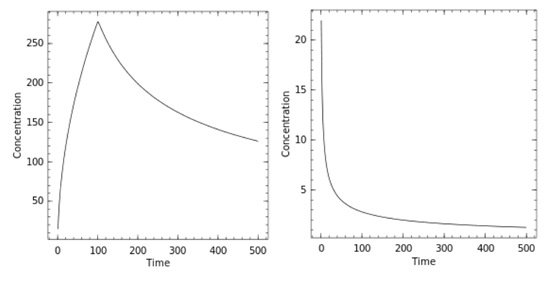
\includegraphics[width=\textwidth]{media/sources.png}
\caption{In each image, the concentration of ligand over time is shown,
  at a distance of one unit from the source. On the left, the instantaneous
  pulse model is used. On the right, the concentration is shown at the
  equivalent location where the emission lasts for 100 steps.}
\end{figure}

The instantaneous pulse model is significantly quicker to compute than the
sustained model because it doesn't require integration.

\begin{figure}[H]
\centering
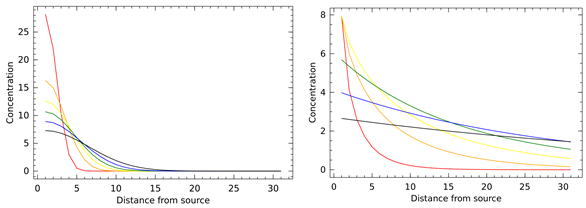
\includegraphics[width=\textwidth]{media/sources2.png}
\caption{The concentration is plotted against the distance from the source
  at time \(t=1\) (red), \(t=3\) 
  (orange), \(t=5\) (yellow), \(t=7\) (green), \(t=10\) (blue) and \(t=15\) (black).
  The left-hand image uses the instantaneous pulse model whereas the right-hand 
  image uses the sustained emission model.} 
\end{figure}

{\bfseries From One Dimension to Two} \\
So that the environmental model has a closer resemblance to real 
biological systems, the CBMP can model sources as a point or as a line. 
To model point-sources, we have made a simplification using the 
separation of the variable technique. This consists of replacing the x2 
by the square distance of the ligand receptor from the source.

{\bfseries Multiple Sources} \\
The user can choose the number of sources and the kind of sources he 
wants as the image of the display of the diffusion window illustrate. 
Each source has its specific parameter input. The parameters are chosen 
in the ligand window. To model the diffusion with more than one source, 
we have assumed that the diffusion is independent of the number of 
sources. Therefore, we add the contribution of each source at each point 
at each time. This simplification allows the algorithm to compute much 
faster, even if it is not physically accurate. The contribution of one 
source at the centre of another source should be equals to zero but in 
our model the concentration of ligand only depends on the distance from 
the source and is thus non-zero. 

{\bfseries The Diffusion Timescale} \\
In writing the CBMP simulator, we have had to take some care to keep the 
diffusion and cell movement on the same timescale. Since one step moves 
with each time increment, if no adjustments were made, then if there are 
more cells, each cell would move slower compared to the ligand. An 
adjustment has been made, so that the amount of time that is understood 
to have passed is determined not just be the number of cell steps taken, 
but also on the number of cells. Thus the diffusion and cell movement 
occur on the same timescale.

\subsection{Collisions -- written by AM and RC, developed by AM}
  Once a cell has a proposed movement, the CBMP 
detects whether the cell with collide with the walls, or any of the 
other cells, and resolves these collisions recursively.

\begin{figure}[H]
\centering
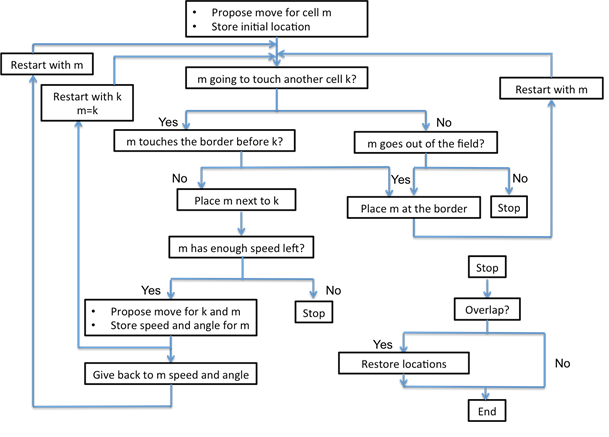
\includegraphics[width=\textwidth]{media/algorithm.png}
\caption{The algorithm for moving cells. To begin with, a move is proposed
for cell m. This move is evaluated by the ballistics functions (in yellow),
which identify whether the cell will collide with another cell, with 
the border, or neither. If there are collisions, then a new move (green) is 
proposed again for any colliding cells and managed recursively. If there
are no collisions, then the cell's move is finished (blue). Once all cells
have finished moving, their locations are given to the overlap-checking routine 
(red) to confirm their locations and declare the movement stage complete.}
\end{figure}

The algorithm for detecting collisions, detailed in Figure 11, begins by storing all of the 
cells' initial location, in case the simulation needs to be restored to 
that original state. The next step is to check 
whether the cell is going to touch any other cells, or to touch the 
border. If the cell has more than one collision in its path, then the 
cell is made to collide with whichever object it would hit first, and 
then the consequences of that collision are played out. 

The first consequence of a collision is that the moving cell is placed 
adjacent to whatever it has collided with. If the cell has momentum to 
bounce off in a new direction, it does so, and it undergoes a new 
movement. In the case of a cell-wall collision, that is all. 
Alternatively, in the case of a collision between two cells, then both 
cells undergo further movement if they have sufficient momentum, and 
this occurs by restarting the algorithm with both cells.

Once all of the cells have settled on new locations and do not have 
sufficient speed to move, one final check is made for any overlaps. If 
there are overlaps, this can suggest that there was an error, such as in 
floating point arithmetic. In the case of an overlap (this occurs less 
than once per 10,000 iterations), the cells are restored to their 
original positions

It is instructive to describe in some more detail how it is detected 
that a cell is colliding with another cell, or that it is colliding with 
the wall.

\subsubsection{Cell-Cell Collisions}
To understand how cell-cell collisions are identified, we can consider 
the most challenging case, where two cells lie on the path of a moving 
cell to its destination. As shown in Figure 12, the moving cell, 
illustrated in black, is denoted m. Its initial position is \(m_0\) 
and its proposed position is \(m_1\). The two cells that lie in its 
path are denoted \(k_1\) and \(k_2\).

\begin{figure}[H]
\centering
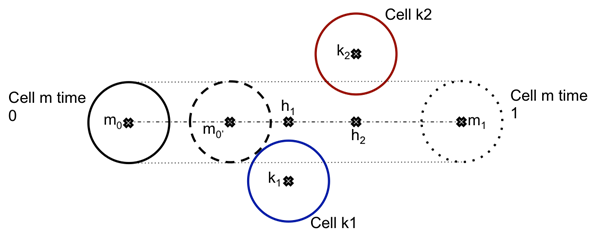
\includegraphics[width=\textwidth]{media/collision.png}
\caption{Cell \(m\) would intersect with two other 
  cells, \(k_1\) and \(k_2\), on the way to its destination. 
  \(m_0\) is its initial position, \(m_1\) is the proposed position and 
\(m_0'\) is its final position.}
\end{figure}

The task of finding where cell \(m\) will first touch another 
cell is divided into four questions:

\begin{enumerate}
\item Which cells lie near enough to the line (of infinite length) that 
passes through \(m_0\) and \(m_1\)
\item Which cells overlap the finite region that \(m\) moves 
through?
\item Where might \(m\) touch those cells?
\item Of those positions, which is the nearest to \(m\)'s 
starting location?
\end{enumerate}

The first question is answered by computing the orthogonal projection \(h_i\) of 
each stationary cell \(k_i\) onto \(\overleftrightarrow{m_0m_1}\), denoted 
\(h_i\). If the distance \(\overline{h_ik_i}\) is less than the sum of the 
radii of both cells (\(\overline{h_ik_i} < r_m + r_{k_i}\)), then the 
stationary cell lies sufficiently close to the path of cell \(m\) to collide 
with it. The length of \(\lvert h_ik_i \rvert\) is given by:

\begin{equation}
\lvert\overline{h_ik_i}\rvert = \frac{\lvert {mx_{k_i} - y_{k_i} + p}\rvert }{\sqrt{1+m^2}}
\end{equation}

where \(y = mx + p\) is the equation of the line passing through \(m_0\)
and \(m_1\), with coefficients:

\begin{equation}
  m = \frac{x_{m_1}-x_{m_0}}{y_{m_1}-y_{m_0}}\text; \qquad p = \frac{-y_{m_1}x_{m_1}+y_{m_0}x_{m_1}}{x_{m_1}-x_{m_0}}
\end{equation}

The second question is answered by ascertaining that the angles \(\angle m_0m_1k_i\) 
and \(\angle m_1m_0k_i\) are both acute, or that 
cell \(k\) is overlapping with \(m\). Both of these angles 
must be acute if \(cos(\measuredangle m_0m_ik\)) and \(cos(\measuredangle m_im_0k)\) are 
both positive, and these cosines can be easily computed 
using the cosine rule.

So far, cells that meet these criteria lie on the the path of cell 
\(m\). However, one needs to decide which of the remaining cells
will be hit by cell \(m\) first. This is done by 
calculating where each of these cells would intersect with the moving 
circumference of cell \(m\), and selecting the collision that is closest to 
\(m\)'s starting point. These possible positions \(m_{0'}\), 
are computed by solving the system:

\begin{equation}
  \begin{cases} 
    y_{m_{0'}} = mx_{m_{0'}} + p \\
    (x_{m_{0'}} - x_{k_i})^2 + (y_{m_{0'}}-y_{k_i})^2 =  (r_m+r_{k_i})^2
  \end{cases}
\end{equation}

Of these solutions for \(m_0\), the one that minimizes \(m_0m_0'\) 
is the true location at which \(m\) must collide with another 
cell. 

As noted previously, once cell \(m\) is moved to \(m_0'\), if 
cells \(m\) and \(k\) have sufficient speed, they will both be assigned new movement vectors.

In a cell-cell collision, a fraction \(g\) of cell \(m\)'s momentum (\(\mathbf{p_m}\)) is conserved and the 
remaining \(1-g\) is lost to the inelasticity of the collision. This means that the final momentum 
of the system (\(\mathbf{p_{system_f}}\)) is equal to \(p_{system_f}\) = \(g) \times p_m\). 
This gives:

\begin{equation}
  gm_m\mathbf{v_0} = m_k\mathbf{v_k}+m_m\mathbf{v_m}
\end{equation}

where \(\mathbf{v_0}\) is the initial velocity of cell \(m\);
\(\mathbf{v_k}\) and \(\mathbf{v_m}\) are the final movement vectors of cells \(m\) and \(k\); and \(m_k\) and
\(m_m\) are the masses of the respective cells.

Moreover, the momentum of the system is split between cells \(m\) and \(k\) as an idealized 
pool-ball collision, as shown in Figure 13. This is a coarse approximation of biological 
reality but is better than the alternative of neglecting to model collisions at all. 

Cell \(k\), which was previously stationary, will 
set out with a movement vector \(\mathbf{v_k}\) in a direction parallel to \(\overrightarrow{m_{0'}k}\).
Cell \(m\) will have a new movement vector \(\mathbf{v_m}\) 
that is perpendicular to \(\mathbf{v_k}\), and whose scalar product with \(\mathbf{v_0}\) 
is positive.

\begin{figure}[H]
\centering
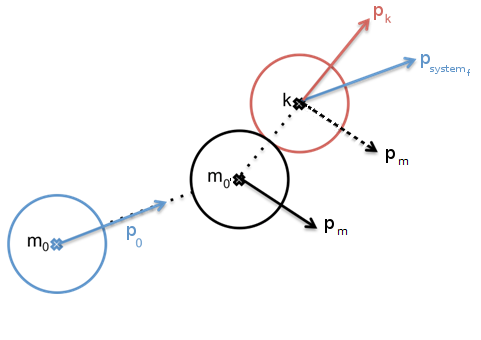
\includegraphics[width=13cm]{media/cellcollide.png}
\caption{Illustration how an angle is selected when cell \(m\) bounces with cell \(k\)}
\end{figure}

The weight of each cell is assumed to be proportional to its squared radius 
as the simulation takes place in a two-dimensional environment, although 
this code can easily be changed if it is desirable to make the mass 
proportional to the cubed radius instead.

\subsubsection{Cell-border Collisions}
The other important kind of collision is between a cell and the border 
of the environment. To put the cell at a border, one needs to know which 
border the cell will touch first. To do this, the first step is to 
calculate the coefficients of the line \(D: y=mx + p\) that passes through 
the cell's starting location and its proposed location. It is not 
sufficient to simply extrapolate \(D\) to the nearest wall (Figure 14). 
Instead, one must equate the line D to the lines 
\(x = x_E) - r_m\), \(x = x_W + r_m\), \(y = y_N - r_m\), \(y = y_S + r_m\), 
where \(x_W\), \(x_E)i\), \(y_N\) and \(y_S\) are the respective \(x\) 
and \(y\) ordinates of each of the four borders.

\begin{figure}[H]
\centering
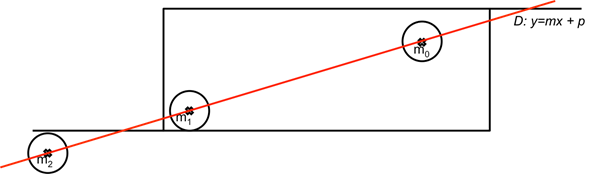
\includegraphics[width=12.98cm]{media/wall.png}
\caption{The challenge of deciding which border m 
  strikes. \(m_0\) is the initial position, \(m_1\)is the final 
  position and \(m_2\)is the proposed position. Note that \(m\) strikes 
  the South wall although the line \(D\) that it is travelling on strikes the 
West wall.}
\end{figure}

This gives a location where the cell-edge would intersect each of the
four borders. To know which border the cell is going to hit 
first, you only look at the two borders that the cell is moving towards, 
and disregard those that are behind. The border that the cell strikes 
first is the one that minimizes the distance \(m_1m_0\), as 
shown in Figure 14. 

The cell can respond to the border in three different ways: 

\begin{enumerate}
  \item If the border is {\itshape reflecting}, then the cell reflects as in optics, 
with a new movement vector that has an outgoing angle the same as the 
incoming angle. The new speed is equal to the original speed minus the distance done
multiplied by g to account for inelasticity. Indeed, as we work with a unitarian time step, 
there are no difference between distance and speed. 
\item If the border is {\itshape absorbing}, then the cell stays at the location \(m_1\), 
  and its speed reduces to zero.
\item If the border is {\itshape removing}, then the cell disappears.
\end{enumerate}

\section{Example Applications --- written by LK and RC, data analysis by RC, images by LK}
The platform has been designed to model diverse biological scenarios with 
slight changes in parameters resulting in large changes in emergent 
behaviour. The precise way that cells respond to ligands in their environment is poorly
understood, \cite{cai} and so the challenge for theoretical biology is to simulate 
this behaviour and use it to suggest what might be driving these cells' behaviour.
The commonality between our models is that a 
chemoattractant is hypothesised that biases cells' behaviour according 
to the concentration gradient established by a ligand source.

Two examples that demonstrate some of the features of the model are:

\begin{itemize}
\item The migration of macrophages to a wound.
\item The behaviour of cells around a stem cell niche
\end{itemize}

These examples are far from exhaustive. For one more example, similar 
applications could arise in modelling the mesenchymal cells present in 
embryogenesis,\cite{caplan91} \cite{merks05} where it has been shown that cells are highly influenced 
by attractive and repulsive chemokines in their local environment.

\subsubsection{Macrophage Migration}
The first model was designed to investigate how macrophages migrate to a 
laceration. This model was designed to copy an experimental setup in 
which lacerations are performed on a fruit fly, and the migration of 
macrophages is microscopically examined on the resultant wound. 
To 
demonstrate how the CBMP could be useful for modelling these data, three 
competing hypotheses were tested. In the first hypothesis, the cell 
migrate towards the wound deterministically. In the second hypothesis, 
the cells are not biased towards the wound at all, but they slow down 
when they get near to it. In the third case, the cells are biased 
towards but their movement towards the wound is stochastic, and they 
again have no particular inclination to slow down when they get there.

In all three simulations, the laceration is modelled as a straight-line 
at the location x=15 and secretes ligands (cytokines) at a constant rate 
for finite duration. The immune cells are initialised to randomly assigned 
locations. The growth rate and death rate are set to zero, and the cells 
are 0.5 units in size. The borders were set to remove stray cells. The 
rest of parameters are available as the preset ``migrate\_random'' and 
``migrate\_non\_random'' models. For each model, ten simulations were 
performed, and their results were analysed as a batch.

In the first model, in which the the cells to be attracted to the wound 
deterministically, they moved to the wound quickly (in 300 timesteps) 
and stayed there for the duration of the simulation. On gross visual 
inspection of this cell motion (Figure 15) and the boxplot that describes 
their distance (Figure 16), the cells move to the laceration more surely 
than would be seen in nature.

\begin{figure}[H]
\centering
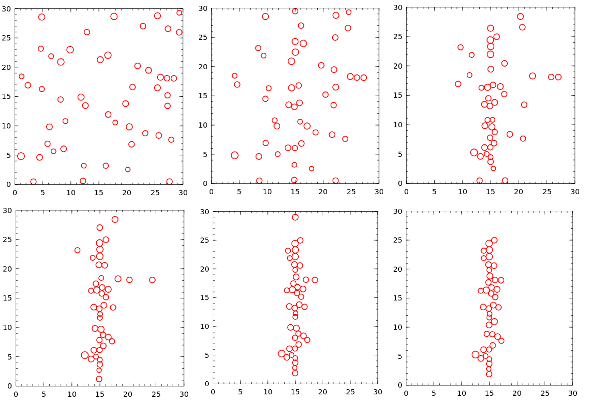
\includegraphics[width=14.41cm]{media/Collated_determinstic.png}
\caption{Shapshots of deterministic 
migration to a laceration at X = 15. Images are shown every 500 timesteps, 
starting at \(t = 1\) (Top left). Cells quickly migrate towards the laceration and 
form a line over the source. T = 3000 is not displayed as there was no 
difference from \(T = 2500\)}
\end{figure}

\begin{figure}[h]
\centering
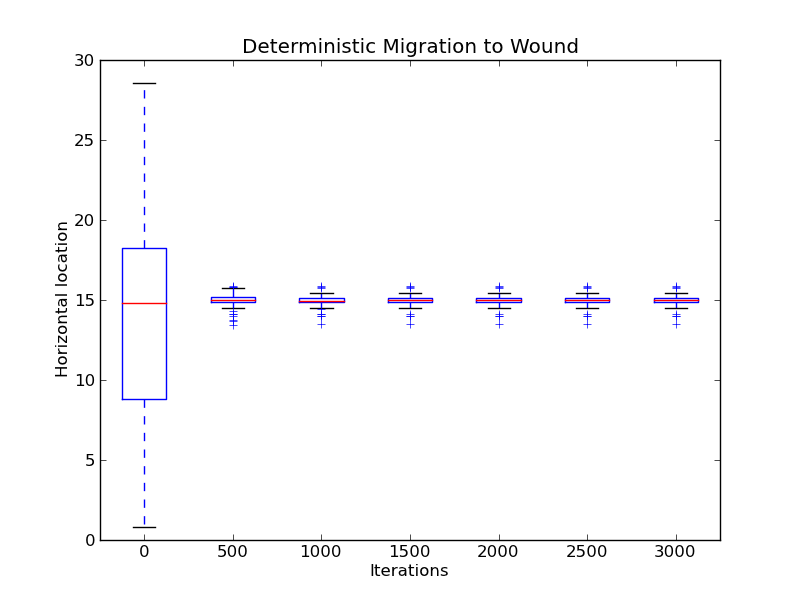
\includegraphics[width=11.51cm]{media/DetMigrationtoWound.png}
\caption{Deterministic migration to the wound, located at \(x=15\). The horizontal location
  of cells over time is shown. Cells rapidly converted to \(x=15\), the 
location of the wound and remain there for the duration of the 
simulation.}
\end{figure}

In the second model, the macrophages were initialised with high 
randomness and no bias, with a tendency to slow down when they neared the 
wound. This simulation provided some evidence macrophages do not arrive 
at wounds solely by being slowed by cytokines or exposed collagen at 
those wounds, as they did not differentially associate at the wound as 
would be expected {\itshape in vivo} (Figure 17). After 3000 timesteps, 
the distribution of cells within the simulation was almost identical, 
with the average position not noticeably closer to the laceration than 
at the beginning of the simulation.
\begin{figure}[H]
\centering
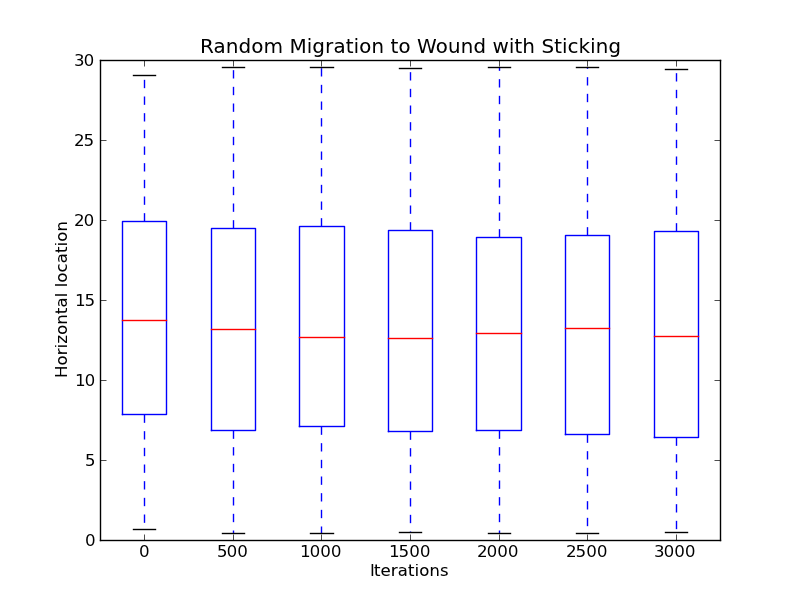
\includegraphics[width=11.51cm]{media/RandomMigrationtoWound.png}
\caption{Random migration with a wound located at \(x=15\). In this simulation, 
  cells are not biased
  to move in one direction more than any other but when they arrive at the wound,
  their motion is slowed. This model did not cause cells to migrate to x=15.
}
\end{figure}

The third simulation provided by far the most realistic results (Figure 18). 
Initialising cells to have a movement pattern made up of equal parts 
persistence, randomness and bias resulted in a slow attraction of cells 
towards the laceration. This is much more representative of the gross 
pattern of behaviour that would be expected in this scenario. Obviously, 
these models are very different and merely aimed to coarsely reproduce 
lifelike dynamics. There may be more insights from comparing more subtly 
different models to the data from automatic microscopy of these 
experiments.

To repeat these simulations, run the platform in GUI mode, and use default
parameters for all values except for the following:

{\itshape Main menu:}
\begin{itemize}
  \item 50 cells
  \item 3000 timesteps
  \item Type of source: Sustained
\end{itemize}
{\itshape Diffusion menu and ligand menu:}
\begin{itemize}
\item Type of source: Line
\item Location: x=15
\item Initial concentration: 100
\item Upper time: 3000
\end{itemize}
{\itshape Cell type:}
\begin{itemize}
  \item For deterministic movement:
    \begin{itemize}
      \item Randomness 0.0
    \end{itemize}
  \item For random movement:
    \begin{itemize}
      \item Randomness 1.0
    \end{itemize}
  \item For stochastic movement:
    \begin{itemize}
      \item Persistence 0.8
      \item Randomness 0.8
    \end{itemize}
\end{itemize}

\begin{figure}[H]
\centering
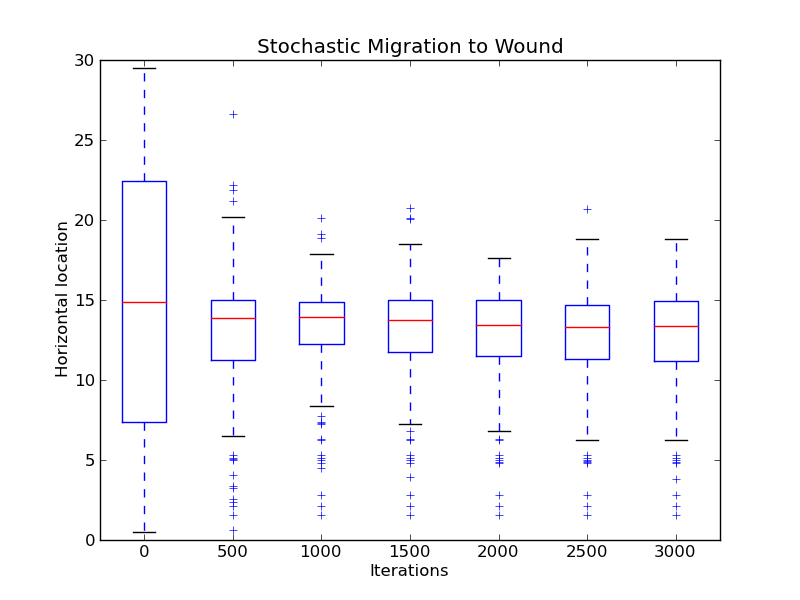
\includegraphics[width=11.51cm]{media/StochMigrationtoWound.png}
\caption{Stochastic migration to the wound, located at \(x=15\). The horizontal location
  of cells over time is shown. Cells rapidly moved to \(x=15\) but some continued to reside
  at a larger distance from the wound source, mostly within five units of the wound.
}
\end{figure}

\subsubsection{Stem Cell Replication}
It is of interest to assess how effectively the CBMP can model the 
dynamics of a stem cell niche because the niche hypothesis has been used 
to describe the dynamics of a wide range of environments, ranging from 
gonadal stem cells in the drosophila ovary to endothelial stem cells in 
mammals.\cite{linheng05} One example that presents a potential experimental 
collaboration for the authors is the case of haematopoeitic stem cells in 
mouse models. Experimental evidence suggests that the Notch1 ligand is 
involved in the expansion of stem cells in a region that is referred to 
as the stem cell niche.\cite{calvi03} In the CBMP model, we defined the stem cell 
niche as the region where the ligand concentration is detected by stem-cells,
so that when they replicate, they are differentially likely to remain as
stem cells. In practice, this 
results in a zone around any designated sources where stem cells grow in 
number. Once outside of this area, any new daughter cells are more 
likely be progenitors. 

To simulate the stem cell niche, we designated stem cells as type 1, 
with a low growth rate of 0.1, a randomness of 0.7 with a persistence of 
0.2 and a concentration response of 1, initialised to the left edge of 
the field. Type 2 cells were designated the progenitors, with a high 
growth rate of 0.2, and randomness of 1.0 but no attraction to the stem 
cell niche. The remainder of parameters can be seen in the {\itshape 
niche\_sim} preset in {\itshape run\_sim.jl}. A constant ligand source can be 
placed as a line or as multiple points along the line \(x=0\) to generate the 
niche; in our simulation, the five units of space on the left hand side 
as the niche, and the rest was designated as non-niche. The borders were 
initialised as the left hand border being absorbing and the other 3 as 
removing. This resulted in the population of stem cells stabilising in 
the niche whilst a population of progenitors was quickly established. 
This population began to drift out of the simulation, creating room for 
new progenitor cells at the stem cell niche border. After about 3500 
iterations the rate of growth of progenitor cells in the field of the 
simulation decreased, and would eventually approach equilibrium (Figure 
19).

\begin{figure}[H]
\centering
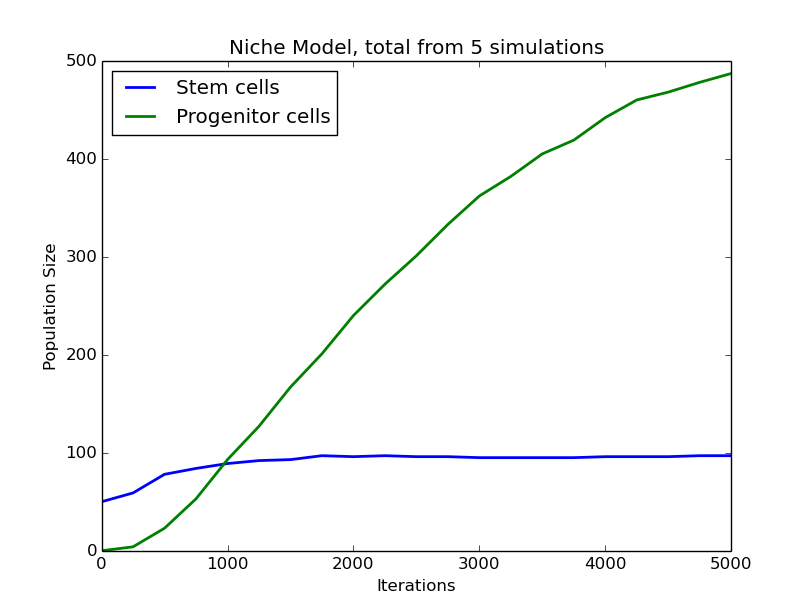
\includegraphics[width=13.51cm]{media/pops.png}
\caption{Stem Cell Niche Simulation. Parameters used: Stem Cells(Blue): Growth Rate: 0.1, Threshold: 0.000793, 
  Persistence: 0.2, Randomness 0.7. Progenitor Cells (Green) Growth Rate: 0.25, Threshold 0.000793, Persistence: 
  0.2, Randomness: 1.0. The stem cell population reaches equilibrium around 2000 timesteps and the progenitor 
cell population does not yet reach stable equilibrium within 5000 timesteps.}
\end{figure}

Figure 20 illustrates how this growth occurs across space.
Initially, the stem cells begin at the leftmost wall of the simulation, 
and they quickly fill out the niche region. Conversely, the progenitor 
cells far outnumber stem cells in the non-niche region, although each 
type of cell spills over to a small degree to the other side of the 
niche boundary.

To repeat this simulation, run the platform in interactive prompt mode 
(run\_sim.jl), using the niche\_sim settings.

\begin{figure}[H]
\centering
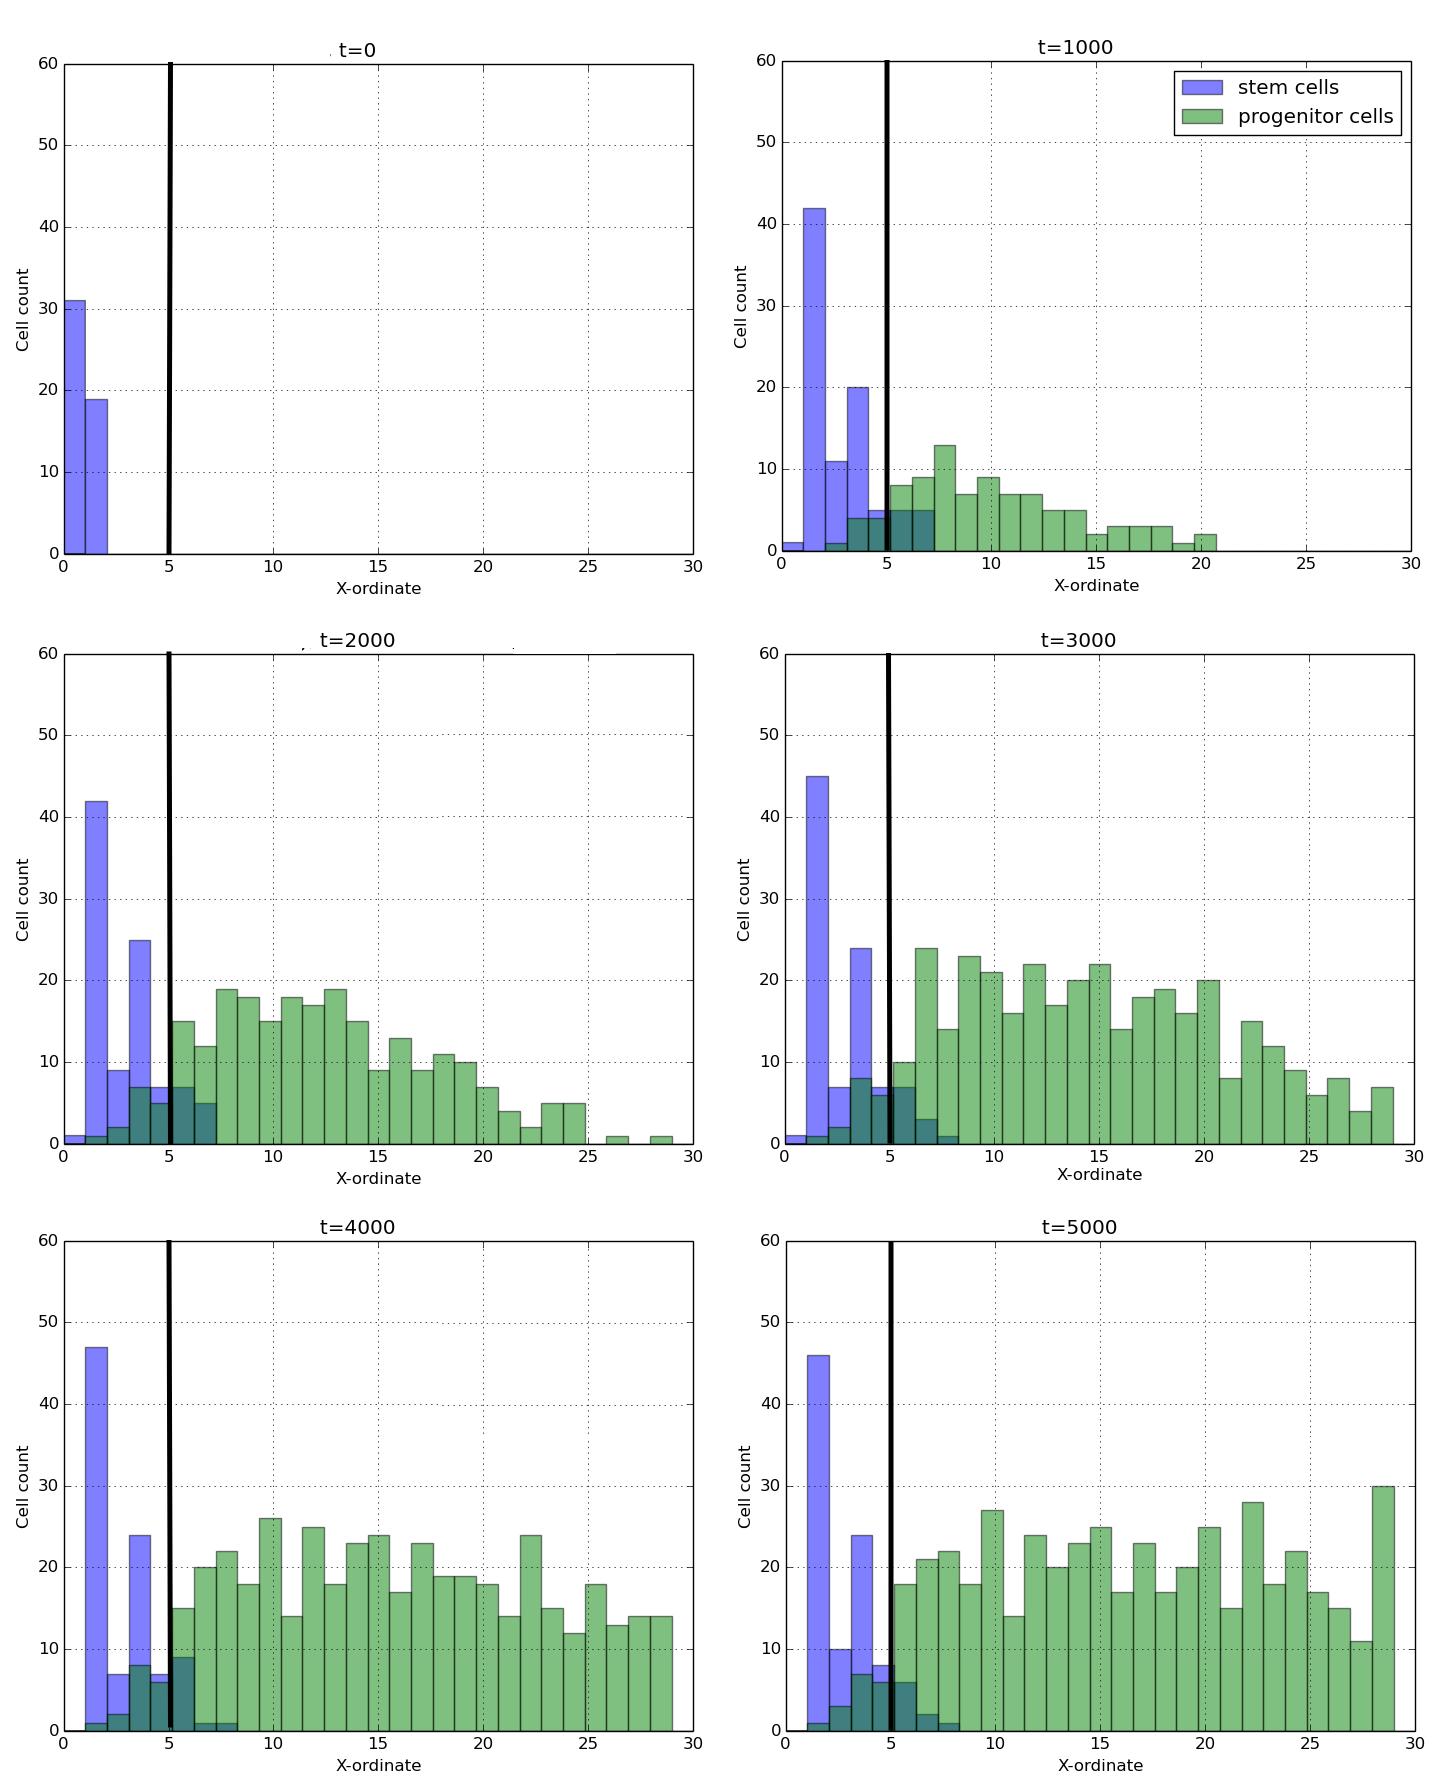
\includegraphics[width=13.51cm]{media/6sim.png}
\caption{Frequency of cells by distance to \(x=0\) in the Stem Cell Niche
  Simulation. The simulation was performed five times, of which all cell 
counts are a total of these runs. The region \(0 \leq x \leq 5\) is 
designated the stem cell niche. The border between the niche and 
non-niche area is indicated by the black vertical line. 
The stem cell population reaches equilibrium around 2000 timesteps 
and the progenitor cell population does not yet reach stable equilibrium 
within 5000 timesteps.
Parameters used: Stem Cells(Blue): Growth Rate: 0.1, Threshold: 25, 
Persistence: 0.2, Randomness 0.7. Progenitor Cells (Green) 
Growth Rate: 0.25, Persistence: 0.2, Randomness: 1.0. 
}
\end{figure}

\section{Performance --- written by RC}
One significant factor that will determine the usefulness of the CBMP, 
especially for the purpose of parameter inference, is its performance. 
On an AMD 1.9GHz single processor desktop computer, the CBMP is able to 
perform 700 iterations per second with a model of sustained ligand 
secretion for twenty cells with eight receptors. This is highly 
dependent on which model is used for diffusion, and how many receptors 
each cell has.

\section{Further Development of the Platform -- written by LK and RC}
For a researcher who can program in Julia, modifications can open up the 
possibility of more diverse models. Alteration to the program's source 
code have been made possible by placing the software on Github, where 
any user can branch it or submit a pull request. The code has been 
commented and moreover, it is logically organised into modules that 
perform specific roles. If a user wants to model cells that decide their 
movement in a different fashion they can alter the move file; if a user 
wants to give the cells more complex characteristics, they can alter the 
Cell type in cell\_type.jl, and so on. The table below can be used to 
ascertain which file or files are needed for any desired alterations 
(Table 1).

\begin{table}[H]
\centering
\begin{tabular}{ll}
\hline
{\bfseries Function} & {\bfseries File(s)} \\
\hline
Cell Properties & cell\_type.jl, gui\_type.jl \\
Diffusion & diffusion.jl, gui\_diffusion.jl \\
Growth, Death and Division & birth\_and\_death.jl \\
Movement & angle.jl, move.jl \\
Command Line & command\_line.jl \\
Process Flow & entry.jl, simulator.jl \\
\hline
\end{tabular}
\caption{Table 1. Platform files and their relevant real world 
functions.}
\end{table}

In ``move.jl'', the function ``tentative\_move'', shown in Figure 21, would plausibly be 
useful to edit, and is an instructive example. Its role is to suggest a 
movement for the cell, that is later modified by any cell-wall or 
cell-cell collisions. However this function may be edited, cells will 
collide as per usual, and will not overlap or exit the bounds of the 
simulation. So users can freely edit the cells' angle or speed on lines 
11 and 16 respectively. Currently, the angle is generated by calling 
{\itshape angle\_from\_both} but instead, one can assign an angle using 
another expression like {\itshape rand()*2pi}, which samples the angle 
from a uniform random distribution. The cell's speed is sampled from a 
Chi-squared distribution (the inverse of this cumulative distribution 
function is given at the start of line 16) but it can easily be changed 
to a constant speed by shortening this line of code to:

{\fontsize{10pt}{10pt} \ttfamily
moving\_cell.speed = categories{[}moving\_cell.cell\_type{]}.avg\_speed} 

This will deterministically assign the same speed to all cells of 
each type. Or to a speed that is proportional to the maximum 
concentration e.g. 

{\fontsize{10pt}{10pt}\ttfamily 
max(concentrations)categories{[}moving\_cell.cell\_type{]}.avg\_speed} 

These are some simple suggestions but much more complex functions are 
feasible.

\begin{figure}[H]
\centering
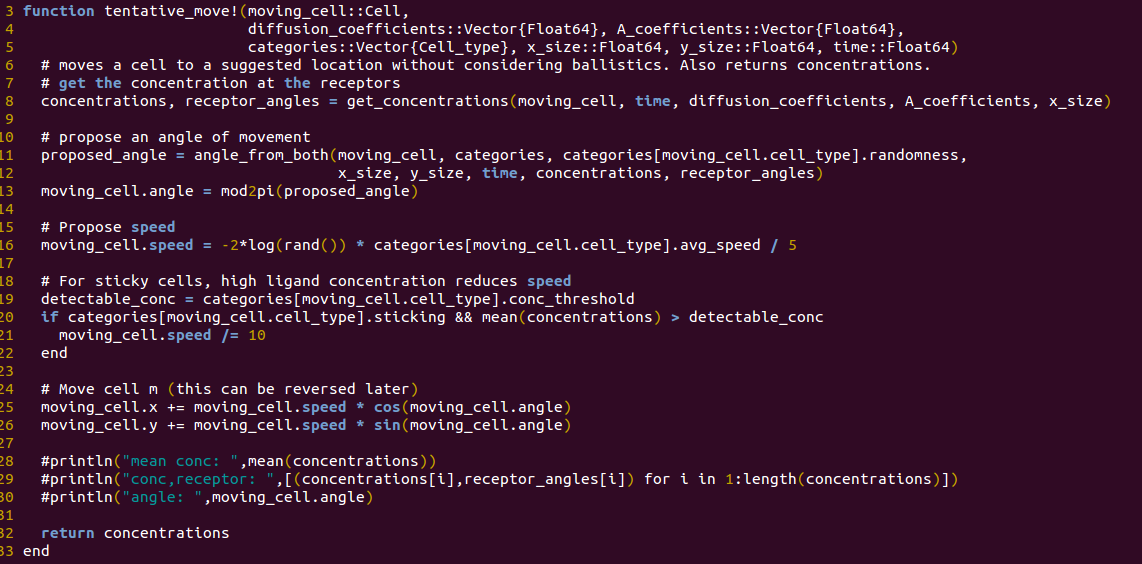
\includegraphics[width=12.23cm]{media/tentativemove.png}
\caption{The tentative\_move function}
\end{figure}

While it has been attempted to make the platform as comprehensive as 
possible, a few powerful developments could not be included in the 
platform, some of which are discussed below. 

First, extensions to the simple implementations of the growth and death 
cellular functions to bring their sophistication in line with movement 
and division would increase the scope of the simulations the platform is 
able to perform. At their most basic, both these functions should be 
linked to local ligand concentration providing growth and survival 
signals. 

This would allow the platform to perform simulations of necrosis and 
potentially preliminary models of migrating mesenchymal cells in 
embryogenesis, where it has been shown the presence of survival signals 
are crucial to the migrational pattern of embryonic cells.\cite{raz09} Implementing 
a distinction between epithelial and mesenchymal cells would work well 
with the aforementioned development, and could all be involved in 
modelling tumour growth and the role of angiogenesis and epithelial to 
mesenchymal transition in the progression of the disease state.

Second, a logical extension of the platform would be to enable it to 
distinguish and keep track of different ligand types throughout the 
environment. This would provide a chance for competing signals to 
influence cellular decisions, which could then be more exquisitely 
responsive to their environment. Another interesting feature would be to 
model how cells respond to secretion of ligand that starts at different 
times. For example, it would be interesting to see how cells react
if they are migrating towards a laceration and then encounter a 
sharp, strong pulse of attractive chemokine. Given that 
the simulation already allows users to specify when each source should 
cease to produce ligand, it would be a small extension to make the 
diffusion start at a time that is also specified by the user, rather 
than at the beginning of the simulation. 

Third, the current method of all cells growing at a type defined rate, 
whilst acceptable, is a huge abstraction from the reality of cellular 
growth. Although this could complicate the model substantially, 
implementing some simple version of the cell cycle in response to 
diverse environmental stimuli would add a lot of functionality to the 
platform. This would allow cells within the same type to be in 
proliferating and nonproliferating phenotypes based on their local 
environment, potentially allowing additional complexity to be added to 
the stem cell niche simulation.

Fourth, it would be beneficial to build a suite to use the simulations 
for parameter inference. The first step in inferring model parameters 
from experimental data would be to set the size of the cells, the field, 
the environment and the timestep appropriately. If these parameters were 
calibrated to an experimental setup, this would allow more careful 
comparison of results produced by the two. The next steps would be more 
complex and interesting - using Bayesian methods, the movement models 
for one or more cells could be calibrated so that the observed behaviour 
is more likely. This inference would have to be restricted to one or two 
parameters, such as the persistence and bias. Either by manual 
exploration or by formal Bayesian inference, the diffusion coefficients 
could also be set to more reasonable values. This could give more 
biological meaning to the relative amounts of ligand predicted in a stem 
cell niche or at an injury.

Fifth, time could be made to advance with a Poisson distribution instead 
of a discrete timescale (e.g. as in Gillespie's Exact Algorithm). 
Currently, the platform uses discrete time steps to iterate through the 
cells in the simulation whilst randomly choosing one cell at a time to 
update. Although this solution works, a more elegant solution would be 
to implement a Poisson distribution to describe the time at which each 
cell moves, with a \(\lambda\) drawn from the number of cells in the simulation at 
the time. This would allow the diffusion equation to update in a more 
natural manner and improve the overall realism of the simulation.

Sixth, it would be beneficial to expand the model to allow ligand to be 
secreted by moving cells. This has immediate biological relevance in the 
case of the haematopoietic stem cell niche, where experimental evidence 
suggests that osteoblastic cells are involved with secreting Notch 
ligand jagged 1, which is involved with maintaining the stem cell niche.
\cite{roeder06}

If user-developers are able to contribute to these facets of the program 
or any others that are useful for their own applications, then they are 
encouraged to submit a pull request to {\itshape 
https://github.com/RyanCarey/abm-platform}, and these will be
promptly actioned. We hope that you enjoy using the software 
and are available to be contacted regarding it using GitHub or via 
email, at ryan.carey14@imperial.ac.uk, 
lewis.kindeleit14@imperial.ac.uk, 
antoine.messager14@imperial.ac.uk.

\section{Conclusion --- written by LK}
The CBMP is an adaptable, extensible platform for modelling diverse cellular behaviours in a user-specified 
environment. It uses an ABM to model cell-behaviour and partial differential equations to model the environment. 
An agent-based approach is ideal for modelling the cells as they are heterogeneous entities with complex 
interactions. For the cytokines, a continuum approach is essential because they are heterogeneous and 
are too numerous to be modelled individually. It can run as a command line interface or as a graphical 
user interface. The command line interface is designed for fast expert use, whereas the GUI has been 
developed to be easier to use, and to display the simulation in real-time. Either interface can output 
the results of simulations as a binary file to allow quantitative analysis in Julia or Python. The platform 
has been developed with a publicly available code-base in Julia, which can readily undergo modification 
by end-users.

There is scope for improving the platform by incorporating new functionality into it. For expert users 
the codebase can be further complicated to carry out a vast array of simulations. The CBMP is already 
helpful for exploring and analysing cellular simulations and will only improve as new additions are made. 

\newpage

\begin{thebibliography}{99}
\bibitem{kaul15}
  Kaul, Himanshu, and Yiannis Ventikos. ``Investigating biocomplexity through the agent-based paradigm.'' {\itshape Briefings in bioinformatics} 16.1 (2015): 137-152. http://bib.oxfordjournals.org/content/16/1/137.full\#ref-2
\bibitem{grimm06} Grimm, Volker, et al. "A standard protocol for describing individual-based and agent-based models." {\itshape Ecological modelling} 198.1 (2006): 115-126.
\bibitem{drasdo07} Drasdo, Dirk, Stefan Hoehme, and Michael Block. "On the role of physics in the growth and pattern formation of multi-cellular systems: What can we learn from individual-cell based models?." {\itshape Journal of Statistical Physics} 128.1-2 (2007): 287-345.]
\bibitem{codling08}
  Codling, Edward A., Michael J. Plank, and Simon Benhamou. ``Random walk models in biology.'' {\itshape Journal of the Royal Society Interface} 5.25 (2008): 813-834.
\bibitem{fick55}
  Fick, Adolph. ``V. On liquid diffusion.'' {\itshape The London, Edinburgh, and Dublin Philosophical Magazine and Journal of Science} 10.63 (1855): 30-39.
\bibitem{cai}
  Cai, Anna Q., Kerry A. Landman, and Barry D. Hughes. ``Modelling directional guidance and motility regulation in cell migration.'' {\itshape Bulletin of mathematical biology} 68.1 (2006): 25-52.
\bibitem{caplan91}
  Caplan, Arnold I. ``Mesenchymal stem cells.'' {\itshape Journal of orthopaedic research} (1991): 641-650.
\bibitem{merks05}
  Merks, Roeland MH, and James A. Glazier. ``A cell-centered approach to developmental biology.'' {\itshape Physica A: Statistical Mechanics and its Applications} 352.1 (2005): 113-130.
\bibitem{linheng05}
  Li, Linheng, and Ting Xie. ``Stem cell niche: structure and function.'' {\itshape Annu. Rev. Cell Dev. Biol.} 21 (2005): 605-631.
\bibitem{calvi03}
  Calvi, L. M., et al. ``Osteoblastic cells regulate the haematopoietic stem cell niche.'' {\itshape Nature} 425.6960 (2003): 841-846.
\bibitem{raz09}
  Raz, Erez, and Harsha Mahabaleshwar. ``Chemokine signaling in embryonic cell migration: a fisheye view.'' {\itshape Development} 136.8 (2009): 1223-1229.
\bibitem{roeder06}
  Roeder, Ingo, et al. ``Dynamic modeling of imatinib-treated chronic myeloid leukemia: functional insights and clinical implications.'' {\itshape Nature medicine} 12.10 (2006): 1181-1184.
\end{thebibliography}

 
%\newpage
%\begin{appendices}
%\end{appendices}

\end{document}
